\section{Cosmology Link --- From Minisuperspace to a Bounce}\label{sec:cosmology}

I sketch classical and quantum pictures in a spatially flat FRW minisuperspace with scale factor $a(t)$ and homogeneous $\theta(t)$.

\subsection{Choice of \texorpdfstring{$I$}{I}: FRW (stiff) vs. WDW (barrier)}\label{sec:i-of-a}
For FRW, take $I=I_0$ (constant). Then
\begin{equation}
\rho_\theta(a) = \frac{\Pi_\theta^2}{2 I_0\,a^6},\qquad \Pi_\theta\equiv a^3\,(I_0\,\dot\theta+q_\theta A_\theta)=\text{const},\quad w=1.
\end{equation}
For WDW, separating $\Psi=\chi(a)e^{i\ell\theta}$ gives a repulsive inverse-square barrier $+\ell^2\hbar^2/(2 I_0 a^2)$.

\subsection{Classical bounce (self-balanced \texorpdfstring{$a^{-6}$}{a-6} and effective potential)}\label{sec:classical-bounce}
Early-time Friedmann with positive shear-like piece $+\Sigma^2/a^6$ and curvature $-k/a^2$ ($k>0$):
\begin{equation}
 H^2 = \frac{8\pi G}{3}\left(\rho_{\mathrm{std}} + \frac{\Pi_\theta^2}{2 I_0\,a^6}\right) + \frac{\Sigma^2}{a^6} - \frac{k}{a^2} \, .
\end{equation}
Defining $A\equiv \tfrac{8\pi G}{3}\tfrac{\Pi_\theta^2}{2I_0}$ and neglecting $\rho_{\mathrm{std}}$ at early times,
\begin{equation}
 H^2=\frac{A+\Sigma^2}{a^6} - \frac{k}{a^2},\qquad a_{\min}=\Big(\frac{A+\Sigma^2}{k}\Big)^{\!1/4} .
\end{equation}

\begin{figure}[htbp]
  \centering
  \begin{subfigure}[b]{0.48\linewidth}
    \centering
  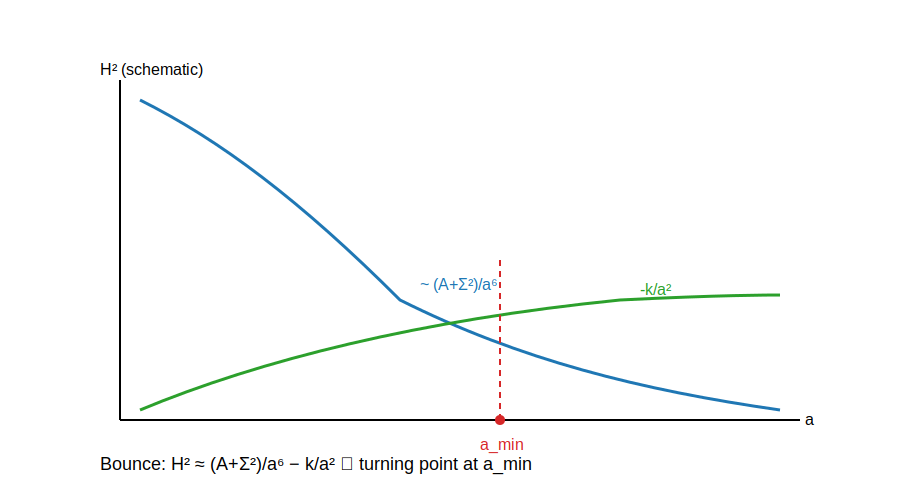
\includegraphics[width=\linewidth]{S4_bounce_schematic.png}
    \caption{Bounce schematic}
    \label{fig:bounce-schematic}
  \end{subfigure}\hfill
  \begin{subfigure}[b]{0.48\linewidth}
    \centering
  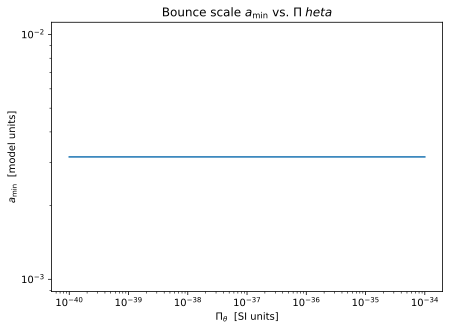
\includegraphics[width=\linewidth]{exp4_bounce_scan.png}
    \caption{Bounce scan (simulation)}
    \label{fig:bounce-scan}
  \end{subfigure}
  \caption{Classical bounce: schematic and simulation turning point.}
  \label{fig:bounce}
\end{figure}

\csvnote{../paper/data/exp4_bounce_scan.csv}

\subsection{Wheeler--DeWitt (quantum) wall at \texorpdfstring{$a=0$}{a=0}}\label{sec:wdw}
Separation $\Psi(a,\theta)=\chi(a)e^{i\ell\theta}$ gives
\begin{equation}
 \left[-\partial_a^2 + U(a) + \frac{\ell^2\hbar^2}{2 I_0 a^2}\right]\chi(a)=0,
\end{equation}
so the $+C/a^2$ term (with $C\propto \ell^2\hbar^2/I_0$) is a repulsive inverse-square barrier. Appropriate boundary conditions (or limit-point behavior for large enough $C$) yield a self-adjoint Hamiltonian and unitary evolution.
